%% ============================================================
%%  §4 生态结构实证
%%  要证明的一句话：
%%    在上游语料中，转换强度收敛于少数"端点"而非层级；成本随硬件家族数增长，
%%    因此"塌缩"在架构层几乎立即发生，在工程层需要十几个到二十几个前端。
%%  素材：docs/04-results-v1.md（五条发现 + 稳健性检验）
%%  建议篇幅：3.5 页（含图 3、图 4、表 2）
%% ============================================================

\section{生态结构实证}
\label{sec:evidence}

%% ---- 方法段（必须先写，且必须交代口径） ----
%% 数据：llvm-project@ba736172 的 mlir/test/**，3329 个 .mlir，181326 个算子。
%% 单元：Conversion/<X>To<Y> 目录 -> 一条层间边；452 个转换文件中 371 个可解析，
%%       81 个因一端方言不定被排除（故 |E| 是下界）。
%% 层划分：5 层 + 跨层通用方言；划分是主观的，已做替代划分的稳健性检验。
%% 一句话必须写：本节统计的是"测试文件数量"，是工程投入分布的代理指标，不是性能、不是使用率。

%% ---- 发现 1：收敛在端点，不在层 ----
%% 79.2% 的层间转换落到最深层（236/298）；但真正的汇聚点是方言：
%% llvm 入度 104、来自 19 个不同方言；其次 rocdl 57、spirv 57。
%% 结论句：共享不是层与层的对称交换，而是所有源指向少数终端的星形结构。
\begin{figure}[t]
  \centering
  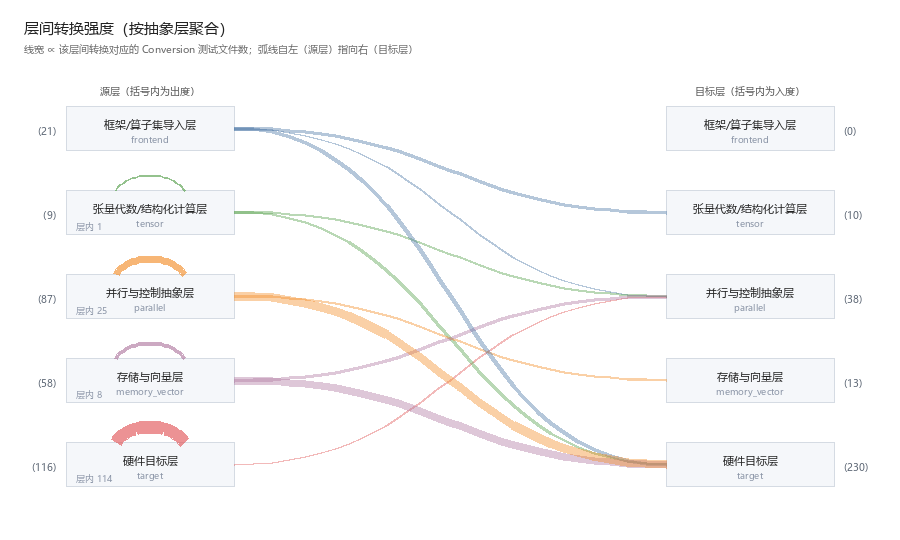
\includegraphics[width=\linewidth]{figures/fig1_layer_transitions.png}
  \caption{层间转换强度（按抽象层聚合）。线宽正比于该层间转换对应的
  \texttt{Conversion} 测试文件数；弧线自左（源层）指向右（目标层）。
  汇入最深层的那束粗线即"端点收敛"。}
  \Description{五层之间的转换弧线图，最右一列入度最大}
  \label{fig:transitions}
\end{figure}

%% ---- 发现 2：厂商在 MLIR 里占两级，不是一层 ----
%% target→target 有 114 个文件 / 8 条边，是全部层间转换中最大的一块：
%% 厂商内二级栈（amdgpu→rocdl 42、xegpu→xevm 20、nvgpu→nvvm 6）与出口转向（spirv→llvm 25 等）。
%% 归因要谨慎：厂商内二级栈只有 3 条边（68 个文件），不是 15→76 膨胀的主因；
%% 主因是层边界内部本身含多个方言对（一条边界平均约 5 个）。

%% ---- 发现 3：投入"两级结构、前端独低"（表 2） ----
\begin{table}[t]
  \caption{各抽象层的测试投入分布。按 \texttt{test/Dialect/<X>} 归属到层；
  跨层通用方言与编译器基础设施方言单列。已归属文件共 1,390 个。}
  \label{tab:investment}
  \small
  \begin{tabularx}{\linewidth}{@{}l S[table-format=3.0] S[table-format=2.1]@{}}
    \toprule
    层 & {文件数} & {占已归属（\%）} \\
    \midrule
    硬件目标层 & 364 & 26.2 \\
    张量代数/结构化计算层 & 354 & 25.5 \\
    并行与控制抽象层 & 235 & 16.9 \\
    存储与向量层 & 222 & 16.0 \\
    跨层通用方言（单列） & 73 & 5.3 \\
    编译器基础设施方言（6 个，单列） & 80 & 5.8 \\
    \textbf{框架/算子集导入层} & \textbf{62} & \textbf{4.5} \\
    \bottomrule
  \end{tabularx}
\end{table}

%% 解释：分布是明显两级——高档（目标 26.2%、张量 25.5%）、中档（并行 16.9%、存储 16.0%）、
%% 低档（导入 4.5%）。导入层只有中后段的约 1/4–1/6。
%% 注意：v1 曾写"四个中后段层几乎均匀（20.6–24.0%）"，那是 Dialect/SparseTensor 与
%% Dialect/LLVMIR 被静默丢弃导致的，已按 review 修正。
%% 原因：承接框架的活在别的仓库（torch-mlir、StableHLO、ONNX-MLIR）；
%% 本语料里 frontend 层作为转换源的方言只有 tosa，torch/stablehlo 一个都没有。

%% ---- 发现 4：两种 |E| 口径，答案相反 ----
%% 架构级 15 个层对 -> N* = 4.6；工程级 76 个方言对 -> N* = 15.5（p=0.6, M=11）。
%% 在 N=8、M=11 时：成对 88 vs 分层 69.2（架构级占优）；88 vs 130.2（工程级更贵）。
%% 敏感性：p 从 1.0 降到 0.4，N* 从 8.7 升到 25.6（约 2.9 倍）。
%% 结论形式必须带条件，不能写成"MLIR 让成本塌缩"。

%% ---- 发现 5：func / arith 是唯一的真·跨层通用语（图 4） ----
\begin{figure}[t]
  \centering
  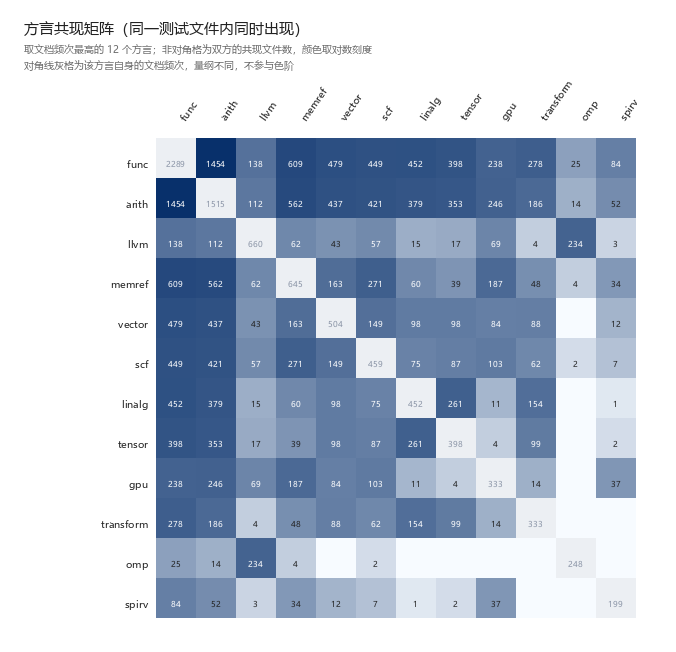
\includegraphics[width=\linewidth]{figures/fig2_dialect_cooccurrence.png}
  \caption{方言共现矩阵（同一测试文件内同时出现）。取文档频次最高的 12 个方言；
  非对角格为双方的共现文件数，颜色取对数刻度；对角线灰格为该方言自身的文档频次，
  量纲不同，不参与色阶。\texttt{func}/\texttt{arith} 与几乎所有层都共现，
  印证其"跨层通用语"地位。}
  \Description{12x12 的方言共现热力图}
  \label{fig:cooccurrence}
\end{figure}

%% ---- 稳健性检验（必须有，证明做过证伪） ----
%% 替代划分（target 拆成通用出口 + 厂商方言，5→6 层）：
%% |E| = 76 与工程级 N* 完全不变；"落到最深层"从 79.2% 掉到 36.6%；非零层对 15→20。
%% 结论：方言级数字是稳的，层级的百分比是划分依赖的 —— 正文只用前者。
